

\subsection{Matrix Method for diphoton channels}

It is widely in use the so called Matrix Method, for signature with two leptons in the final state. The Matrix Method generally estimates the various background contributions and the signal contribution according to their real and fake content of objects in the event. This is done by applying a matrix version inversion which solves a linear system of equations in which the unknowns are the background and signal components, while the known values are the yields three levels of selection (a tight, a medium and a loose selection) and the coefficient of linearity of the system, that are expressed in terms of the object faka rates and signal efficiencies.

In the diphoton channels the Matrix Method cannot be simply applied as in the case of the dilepton channel. This is due to the fact that the sources of fake photons are essentially three: fake photons from quarks, from gluons and fake photons from leptons. We need therefore to explcitily write down all the contributions to the various levels of selection:

\begin{eqnarray}
N_{L} & = & \left( N_{L}^{lq} + N_{L}^{lg} + N_{L}^{ll} + N_{L}^{qq} + N_{L}^{gg} + N_{L}^{qg} \right) + \left( N_{L}^{sq} + N_{L}^{sg} + N_{L}^{sl} \right) + N_{L}^{ss}, \label{eq:mm1_}\\
N_{M} & = & \left( N_{M}^{lq} + N_{M}^{lg} + N_{M}^{ll} + N_{M}^{qq} + N_{M}^{gg} + N_{M}^{qg} \right) + \left( N_{M}^{sq} + N_{M}^{sg} + N_{M}^{sl} \right) + N_{M}^{ss}, \label{eq:mm2_}\\
N_{T} & = & \left( N_{T}^{lq} + N_{T}^{lg} + N_{T}^{ll} + N_{T}^{qq} + N_{T}^{gg} + N_{T}^{qg} \right) + \left( N_{T}^{sq} + N_{T}^{sg} + N_{T}^{sl} \right) + N_{T}^{ss}. \label{eq:mm3_}
\end{eqnarray}

Here we indicate with $l$ the fake photons from leptons, with $q$ and $g$ the fake photons from quarks and gluons, respectively, and with $s$ the real (signal) photons. Therefore for instance $N_{L}^{lj}$ will be the number of events selected by the loose isolation which have one fake photon from lepton and one fake photon from jet in the final state. While $N_{L}^{sl}$ will be the number of loosely selected events with one real and one fake from lepton final state photon. As it can be noticed, all the same type of events have been grouped according to whether they have 2 fake, 1 real and 1 fake or 2 real final state photons. This categorization suggests the following definitions:

\begin{eqnarray}
N_{L(M)(T)}^{ff} & \equiv & N_{L(M)(T)}^{lq} + N_{L(M)(T)}^{lg} + N_{L(M)(T)}^{ll} + N_{L(M)(T)}^{qq} + N_{L(M)(T)}^{gg} + N_{L(M)(T)}^{qg}, \label{eq:N1_}\\
N_{L(M)(T)}^{sf} & \equiv & N_{L(M)(T)}^{sq} + N_{L(M)(T)}^{sg} + N_{L(M)(T)}^{sl}. \label{eq:N2_}
\end{eqnarray}

\begin{eqnarray}
\epsilon_{ff}^{L \rightarrow M(T)} & \equiv & \frac{N_{M(T)}^{ff}}{N_{L}^{ff}}, \label{eq:eps1_}\\
\epsilon_{sf}^{L \rightarrow M(T)} & \equiv & \frac{N_{M(T)}^{sf}}{N_{L}^{sf}}, \label{eq:eps2_}\\
\epsilon_{ss}^{L \rightarrow M(T)} & \equiv & \frac{N_{M(T)}^{ss}}{N_{L}^{ss}}. \label{eq:eps3_}
\end{eqnarray}

Therefore, the system of equations can be rewritted as:

\begin{eqnarray}
N_{L} & = & N_{L}^{ff} + N_{L}^{sf} + N_{L}^{ss}, \label{eq:mm4_}\\
N_{M} & = & \epsilon_{ff}^{L \rightarrow M} N_{L}^{ff} + \epsilon_{sf}^{L \rightarrow M} N_{L}^{sf} + \epsilon_{ss}^{L \rightarrow M} N_{L}^{ss}, \label{eq:mm5_}\\
N_{T} & = & \epsilon_{ff}^{L \rightarrow T} N_{L}^{ff} + \epsilon_{sf}^{L \rightarrow T} N_{L}^{sf} + \epsilon_{ss}^{L \rightarrow T} N_{L}^{ss}. \label{eq:mm6_}
\end{eqnarray}

And the components of the $\epsilon$s:

\begin{eqnarray}
\epsilon_{lq}^{L \rightarrow M(T)} & \equiv & \frac{N_{M(T)}^{lq}}{N_{L}^{ff}}, \label{eq:eps4_}\\
\epsilon_{lg}^{L \rightarrow M(T)} & \equiv & \frac{N_{M(T)}^{lg}}{N_{L}^{ff}}, \label{eq:eps4__}\\
\epsilon_{ll}^{L \rightarrow M(T)} & \equiv & \frac{N_{M(T)}^{ll}}{N_{L}^{ff}}, \label{eq:eps5_}\\
\epsilon_{qq}^{L \rightarrow M(T)} & \equiv & \frac{N_{M(T)}^{qq}}{N_{L}^{ff}}, \label{eq:eps6__}\\
\epsilon_{gg}^{L \rightarrow M(T)} & \equiv & \frac{N_{M(T)}^{gg}}{N_{L}^{ff}}, \label{eq:eps6___}\\
\epsilon_{qg}^{L \rightarrow M(T)} & \equiv & \frac{N_{M(T)}^{qg}}{N_{L}^{ff}}, \label{eq:eps6____}\\
\epsilon_{sq}^{L \rightarrow M(T)} & \equiv & \frac{N_{M(T)}^{sq}}{N_{L}^{sf}}, \label{eq:eps7}\\
\epsilon_{sg}^{L \rightarrow M(T)} & \equiv & \frac{N_{M(T)}^{sg}}{N_{L}^{sf}}, \label{eq:eps8}\\
\epsilon_{sl}^{L \rightarrow M(T)} & \equiv & \frac{N_{M(T)}^{sl}}{N_{L}^{sf}}. \label{eq:eps8_}
\end{eqnarray}


These are those which we can call component $\epsilon$s. We can indeed write:

\begin{eqnarray}
\epsilon_{ff}^{L \rightarrow M(T)} & = & \epsilon_{lq}^{L \rightarrow M(T)} + \epsilon_{lg}^{L \rightarrow M(T)} + \epsilon_{ll}^{L \rightarrow M(T)} + \epsilon_{qq}^{L \rightarrow M(T)} + \epsilon_{gg}^{L \rightarrow M(T)} + \epsilon_{qg}^{L \rightarrow M(T)},\label{eq:eps9_} \\ 
\epsilon_{sf}^{L \rightarrow M(T)} & = & \epsilon_{sq}^{L \rightarrow M(T)} + \epsilon_{sg}^{L \rightarrow M(T)} + \epsilon_{sl}^{L \rightarrow M(T)}. \label{eq:eps10_}
\end{eqnarray}

Let's now work out the detailed expression of the component $\epsilon$s:

\begin{eqnarray}
\epsilon_{lq}^{L \rightarrow T} & = & \frac{N_{T}^{lq}}{N_{L}^{lq}+N_{L}^{lg}+N_{L}^{ll}+N_{L}^{qq}+N_{L}^{gg}+N_{L}^{qg}} =
\frac{N_{T}^{lq}}{N_{L}^{lq}} \cdot \frac{1}{1 + \frac{N_{L}^{lg}}{N_{L}^{lq}} + \frac{N_{L}^{ll}}{N_{L}^{lq}} + \frac{N_{L}^{qq}}{N_{L}^{lq}} + \frac{N_{L}^{gg}}{N_{L}^{lq}} + \frac{N_{L}^{qg}}{N_{L}^{lq}}} \nonumber \\
& = & \epsilon_{l} \epsilon_{q} \cdot \frac{1}{1 + R^{lg/lq} + R^{ll/lq} + R^{qq/lq} + R^{gg/lq} + R^{qg/lq}}, \label{eq:eps11_}\\
\epsilon_{lg}^{L \rightarrow T} & = & \frac{N_{T}^{lg}}{N_{L}^{lq}+N_{L}^{lg}+N_{L}^{ll}+N_{L}^{qq}+N_{L}^{gg}+N_{L}^{qg}} =
\frac{N_{T}^{lg}}{N_{L}^{lg}} \cdot \frac{1}{1 + \frac{N_{L}^{lq}}{N_{L}^{lg}} + \frac{N_{L}^{ll}}{N_{L}^{lg}} + \frac{N_{L}^{qq}}{N_{L}^{lg}} + \frac{N_{L}^{gg}}{N_{L}^{lg}} + \frac{N_{L}^{qg}}{N_{L}^{lg}}} \nonumber \\
& = & \epsilon_{l} \epsilon_{g} \cdot \frac{1}{1 + R^{lq/lg} + R^{ll/lg} + R^{qq/lg} + R^{gg/lg} + R^{qg/lg}}, \label{eq:eps12_}\\
\epsilon_{ll}^{L \rightarrow T} & = & \frac{N_{T}^{ll}}{N_{L}^{lq}+N_{L}^{lg}+N_{L}^{ll}+N_{L}^{qq}+N_{L}^{gg}+N_{L}^{qg}} =
\frac{N_{T}^{ll}}{N_{L}^{ll}} \cdot \frac{1}{1 + \frac{N_{L}^{lq}}{N_{L}^{ll}} + \frac{N_{L}^{lg}}{N_{L}^{ll}} + \frac{N_{L}^{qq}}{N_{L}^{ll}} + \frac{N_{L}^{gg}}{N_{L}^{ll}} + \frac{N_{L}^{qg}}{N_{L}^{ll}}} \nonumber \\
& = & \epsilon_{l}^{2} \cdot \frac{1}{1 + R^{lq/ll} + R^{lg/ll} + R^{qq/ll} + R^{gg/ll} + R^{qg/ll}}, \label{eq:eps13_}\\
\epsilon_{qq}^{L \rightarrow T} & = & \frac{N_{T}^{qq}}{N_{L}^{lq}+N_{L}^{lg}+N_{L}^{ll}+N_{L}^{qq}+N_{L}^{gg}+N_{L}^{qg}} =
\frac{N_{T}^{qq}}{N_{L}^{qq}} \cdot \frac{1}{1 + \frac{N_{L}^{lq}}{N_{L}^{qq}} + \frac{N_{L}^{lg}}{N_{L}^{qq}} + \frac{N_{L}^{ll}}{N_{L}^{qq}} + \frac{N_{L}^{gg}}{N_{L}^{qq}} + \frac{N_{L}^{qg}}{N_{L}^{qq}}} \nonumber \\
& = & \epsilon_{q}^{2} \cdot \frac{1}{1 + R^{lq/qq} + R^{lg/qq} + R^{ll/qq} + R^{gg/qq} + R^{qg/qq}}, \label{eq:eps14_}\\
\epsilon_{gg}^{L \rightarrow T} & = & \frac{N_{T}^{gg}}{N_{L}^{lq}+N_{L}^{lg}+N_{L}^{ll}+N_{L}^{qq}+N_{L}^{gg}+N_{L}^{qg}} =
\frac{N_{T}^{gg}}{N_{L}^{gg}} \cdot \frac{1}{1 + \frac{N_{L}^{lq}}{N_{L}^{gg}} + \frac{N_{L}^{lg}}{N_{L}^{gg}} + \frac{N_{L}^{ll}}{N_{L}^{gg}} + \frac{N_{L}^{qq}}{N_{L}^{gg}} + \frac{N_{L}^{qg}}{N_{L}^{gg}}} \nonumber \\
& = & \epsilon_{g}^{2} \cdot \frac{1}{1 + R^{lq/gg} + R^{lg/gg} + R^{ll/gg} + R^{qq/gg} + R^{qg/gg}}, \label{eq:eps15_}\\
\epsilon_{qg}^{L \rightarrow T} & = & \frac{N_{T}^{qg}}{N_{L}^{lq}+N_{L}^{lg}+N_{L}^{ll}+N_{L}^{qq}+N_{L}^{gg}+N_{L}^{qg}} =
\frac{N_{T}^{qg}}{N_{L}^{qg}} \cdot \frac{1}{1 + \frac{N_{L}^{lq}}{N_{L}^{qg}} + \frac{N_{L}^{lg}}{N_{L}^{qg}} + \frac{N_{L}^{ll}}{N_{L}^{qg}} + \frac{N_{L}^{qq}}{N_{L}^{qg}} + \frac{N_{L}^{gg}}{N_{L}^{qg}}} \nonumber \\
& = & \epsilon_{q} \epsilon_{g} \cdot \frac{1}{1 + R^{lq/qg} + R^{lg/qg} + R^{ll/qg} + R^{qq/qg} + R^{gg/qg}}, \label{eq:eps16_}
\end{eqnarray}

\begin{eqnarray}
\epsilon_{lq}^{L \rightarrow M} & = & \frac{N_{M}^{lq}}{N_{L}^{lq}+N_{L}^{lg}+N_{L}^{ll}+N_{L}^{qq}+N_{L}^{gg}+N_{L}^{qg}} =
\frac{N_{M}^{lq}}{N_{L}^{lq}} \cdot \frac{1}{1 + \frac{N_{L}^{lg}}{N_{L}^{lq}} + \frac{N_{L}^{ll}}{N_{L}^{lq}} + \frac{N_{L}^{qq}}{N_{L}^{lq}} + \frac{N_{L}^{gg}}{N_{L}^{lq}} + \frac{N_{L}^{qg}}{N_{L}^{lq}}} \nonumber \\
& = & \left( \epsilon_{l} + \epsilon_{q} - \epsilon_{l} \epsilon_{q} \right) \cdot \frac{1}{1 + R^{lg/lq} + R^{ll/lq} + R^{qq/lq} + R^{gg/lq} + R^{qg/lq}}, \label{eq:eps11_}\\
\epsilon_{lg}^{L \rightarrow M} & = & \frac{N_{M}^{lg}}{N_{L}^{lq}+N_{L}^{lg}+N_{L}^{ll}+N_{L}^{qq}+N_{L}^{gg}+N_{L}^{qg}} =
\frac{N_{M}^{lg}}{N_{L}^{lg}} \cdot \frac{1}{1 + \frac{N_{L}^{lq}}{N_{L}^{lg}} + \frac{N_{L}^{ll}}{N_{L}^{lg}} + \frac{N_{L}^{qq}}{N_{L}^{lg}} + \frac{N_{L}^{gg}}{N_{L}^{lg}} + \frac{N_{L}^{qg}}{N_{L}^{lg}}} \nonumber \\
& = & \left( \epsilon_{l} + \epsilon_{g} - \epsilon_{l} \epsilon_{g} \right) \cdot \frac{1}{1 + R^{lq/lg} + R^{ll/lg} + R^{qq/lg} + R^{gg/lg} + R^{qg/lg}}, \label{eq:eps12__}\\
\epsilon_{ll}^{L \rightarrow M} & = & \frac{N_{M}^{ll}}{N_{L}^{lq}+N_{L}^{lg}+N_{L}^{ll}+N_{L}^{qq}+N_{L}^{gg}+N_{L}^{qg}} =
\frac{N_{M}^{ll}}{N_{L}^{ll}} \cdot \frac{1}{1 + \frac{N_{L}^{lq}}{N_{L}^{ll}} + \frac{N_{L}^{lg}}{N_{L}^{ll}} + \frac{N_{L}^{qq}}{N_{L}^{ll}} + \frac{N_{L}^{gg}}{N_{L}^{ll}} + \frac{N_{L}^{qg}}{N_{L}^{ll}}} \nonumber \\
& = & \left( 2 \epsilon_{l} - \epsilon_{l}^{2} \right) \cdot \frac{1}{1 + R^{lq/ll} + R^{lg/ll} + R^{qq/ll} + R^{gg/ll} + R^{qg/ll}}, \label{eq:eps13__}\\
\epsilon_{qq}^{L \rightarrow M} & = & \frac{N_{M}^{qq}}{N_{L}^{lq}+N_{L}^{lg}+N_{L}^{ll}+N_{L}^{qq}+N_{L}^{gg}+N_{L}^{qg}} =
\frac{N_{M}^{qq}}{N_{L}^{qq}} \cdot \frac{1}{1 + \frac{N_{L}^{lq}}{N_{L}^{qq}} + \frac{N_{L}^{lg}}{N_{L}^{qq}} + \frac{N_{L}^{ll}}{N_{L}^{qq}} + \frac{N_{L}^{gg}}{N_{L}^{qq}} + \frac{N_{L}^{qg}}{N_{L}^{qq}}} \nonumber \\
& = & \left( 2 \epsilon_{q} - \epsilon_{q}^{2} \right) \cdot \frac{1}{1 + R^{lq/qq} + R^{lg/qq} + R^{ll/qq} + R^{gg/qq} + R^{qg/qq}}, \label{eq:eps14__}\\
\epsilon_{gg}^{L \rightarrow M} & = & \frac{N_{M}^{gg}}{N_{L}^{lq}+N_{L}^{lg}+N_{L}^{ll}+N_{L}^{qq}+N_{L}^{gg}+N_{L}^{qg}} =
\frac{N_{M}^{gg}}{N_{L}^{gg}} \cdot \frac{1}{1 + \frac{N_{L}^{lq}}{N_{L}^{gg}} + \frac{N_{L}^{lg}}{N_{L}^{gg}} + \frac{N_{L}^{ll}}{N_{L}^{gg}} + \frac{N_{L}^{qq}}{N_{L}^{gg}} + \frac{N_{L}^{qg}}{N_{L}^{gg}}} \nonumber \\
& = & \left( 2 \epsilon_{g} - \epsilon_{g}^{2} \right) \cdot \frac{1}{1 + R^{lq/gg} + R^{lg/gg} + R^{ll/gg} + R^{qq/gg} + R^{qg/gg}}, \label{eq:eps15__}\\
\epsilon_{qg}^{L \rightarrow M} & = & \frac{N_{M}^{qg}}{N_{L}^{lq}+N_{L}^{lg}+N_{L}^{ll}+N_{L}^{qq}+N_{L}^{gg}+N_{L}^{qg}} =
\frac{N_{M}^{qg}}{N_{L}^{qg}} \cdot \frac{1}{1 + \frac{N_{L}^{lq}}{N_{L}^{qg}} + \frac{N_{L}^{lg}}{N_{L}^{qg}} + \frac{N_{L}^{ll}}{N_{L}^{qg}} + \frac{N_{L}^{qq}}{N_{L}^{qg}} + \frac{N_{L}^{gg}}{N_{L}^{qg}}} \nonumber \\
& = & \left( \epsilon_{q} + \epsilon_{g} - \epsilon_{q} \epsilon_{g} \right) \cdot \frac{1}{1 + R^{lq/qg} + R^{lg/qg} + R^{ll/qg} + R^{qq/qg} + R^{gg/qg}}, \label{eq:eps16__}
\end{eqnarray}

\begin{eqnarray}
\epsilon_{sq}^{L \rightarrow T} & = & \frac{N_{T}^{sq}}{N_{L}^{sq}+N_{L}^{sg}+N_{L}^{sl}} = \frac{N_{T}^{sq}}{N_{L}^{sq}} \cdot \frac{1}{1 + \frac{N_{L}^{sg}}{N_{L}^{sq}} + \frac{N_{L}^{sl}}{N_{L}^{sq}}} \nonumber \\
& = & \epsilon_{s} \epsilon_{q} \cdot \frac{1}{1 + R^{sg/sq} + R^{sl/sq}}, \label{eq:eps17_}\\
\epsilon_{sg}^{L \rightarrow T} & = & \frac{N_{T}^{sg}}{N_{L}^{sq}+N_{L}^{sg}+N_{L}^{sl}} = \frac{N_{T}^{sg}}{N_{L}^{sg}} \cdot \frac{1}{1 + \frac{N_{L}^{sq}}{N_{L}^{sg}} + \frac{N_{L}^{sl}}{N_{L}^{sg}}} \nonumber \\
& = & \epsilon_{s} \epsilon_{g} \cdot \frac{1}{1 + R^{sq/sg} + R^{sl/sg}}, \label{eq:eps17__}\\
\epsilon_{sl}^{L \rightarrow T} & = & \frac{N_{T}^{sl}}{N_{L}^{sq}+N_{L}^{sg}+N_{L}^{sl}} = \frac{N_{T}^{sl}}{N_{L}^{sl}} \cdot \frac{1}{1 + \frac{N_{L}^{sq}}{N_{L}^{sl}} + \frac{N_{L}^{sg}}{N_{L}^{sl}}} \nonumber \\
& = & \epsilon_{s} \epsilon_{l} \cdot \frac{1}{1 + R^{sq/sl} + R^{sg/sl}}, \label{eq:eps17___}\\
\epsilon_{sq}^{L \rightarrow M} & = & \frac{N_{M}^{sq}}{N_{L}^{sq}+N_{L}^{sg}+N_{L}^{sl}} = \frac{N_{M}^{sq}}{N_{L}^{sq}} \cdot \frac{1}{1 + \frac{N_{L}^{sg}}{N_{L}^{sq}} + \frac{N_{L}^{sl}}{N_{L}^{sq}}} \nonumber \\
& = & \left( \epsilon_{s} + \epsilon_{q} - \epsilon_{s} \epsilon_{q} \right) \cdot \frac{1}{1 + R^{sg/sq} + R^{sl/sq}}, \label{eq:eps18_}\\
\epsilon_{sg}^{L \rightarrow M} & = & \frac{N_{M}^{sg}}{N_{L}^{sq}+N_{L}^{sg}+N_{L}^{sl}} = \frac{N_{M}^{sg}}{N_{L}^{sg}} \cdot \frac{1}{1 + \frac{N_{L}^{sq}}{N_{L}^{sg}} + \frac{N_{L}^{sl}}{N_{L}^{sg}}} \nonumber \\
& = & \left( \epsilon_{s} + \epsilon_{g} - \epsilon_{s} \epsilon_{g} \right) \cdot \frac{1}{1 + R^{sq/sg} + R^{sl/sg}}, \label{eq:eps18__}\\
\epsilon_{sl}^{L \rightarrow M} & = & \frac{N_{M}^{sl}}{N_{L}^{sq}+N_{L}^{sg}+N_{L}^{sl}} = \frac{N_{M}^{sl}}{N_{L}^{sl}} \cdot \frac{1}{1 + \frac{N_{L}^{sq}}{N_{L}^{sl}} + \frac{N_{L}^{sg}}{N_{L}^{sl}}} \nonumber \\
& = & \left( \epsilon_{s} + \epsilon_{l} - \epsilon_{s} \epsilon_{l} \right) \cdot \frac{1}{1 + R^{sq/sl} + R^{sg/sl}}, \label{eq:eps18___}\\
\epsilon_{ss}^{L \rightarrow T} & = & \frac{N_{T}^{ss}}{N_{L}^{ss}} = \epsilon_{s}^2, \label{eq:eps21_}\\
\epsilon_{ss}^{L \rightarrow M} & = & \frac{N_{M}^{ss}}{N_{L}^{ss}} = 2 \epsilon_{s} - \epsilon_{s}^2. \label{eq:eps22_}
\end{eqnarray}

where the ratio factors $R^{xy/st}$ are defined as following:

\begin{eqnarray}
R^{xy/st} \equiv \frac{N_{L}^{xy}}{N_{L}^{st}}. \label{eq:R1}
\end{eqnarray}

For more details see \cite{MMDiphotonAN}.

As it can be noticed, the system of equations can be solved once the object-level efficiencies ($\epsilon_l$, $\epsilon_q$, $\epsilon_g$, $\epsilon_s$) and the ratio factors, have been estimated from data. It can also be noticed that, given the properties of the ratio factors, they can all be expressed in terms of a set of seven of them, for instance: $R^{sl/sq}$, $R^{sl/sg}$, $R^{qg/lq}$, $R^{qg/lg}$, $R^{qg/ll}$, $R^{qg/qq}$, $R^{qg/gg}$.


In practice we estimate $\epsilon_l$ from a Tag and Probe technique on an electron-photon couple of objects. We estimate $\epsilon_q$, $\epsilon_g$ thanks to a template fitting procedure. We estimate $\epsilon_s$ thanks to a Tag and Probe technique, by fitting the invariant mass of the di-muon gamma system. Finally the ratio factors will be estimated by counting the number of two object events in the signal region.


\subsubsection{Application of the Matrix Method to the $T^{*}$ Diphoton channel}

As we have seen, in order to estimate the number of background events containing one or two fake photons from data, we need to estimate the efficiency and ratio factors from data. In the following subsections we will describe the 
procedur
e to obtain from data, the ratio factors, the fake rate from jets (produced by the hadronization of quark-like and gluon-like partons), from leptons and the real photon efficiency.

\subsubsubsection{Photon Fake Rate from leptons}

First of all we would like to stress that the so called $\epsilon$s are defined to be a ratio of fake rates (or signal efficiencies), therefore should be seen as a relative fake rate. In the specific case of the fake rate from 
leptons, we
 define the $\epsilon_{l}$ as the per-object ratio of the photon fake rate for the tight selection over the fake rate for the no-electron-veto selection. Where the tight selection is the usual tight ID photon selection, while the 
no-electron-veto selection will be the tight ID selection with the exception of the electron-veto cut.

\begin{figure}[!ht]
  \begin{center}
       \resizebox{10cm}{!}{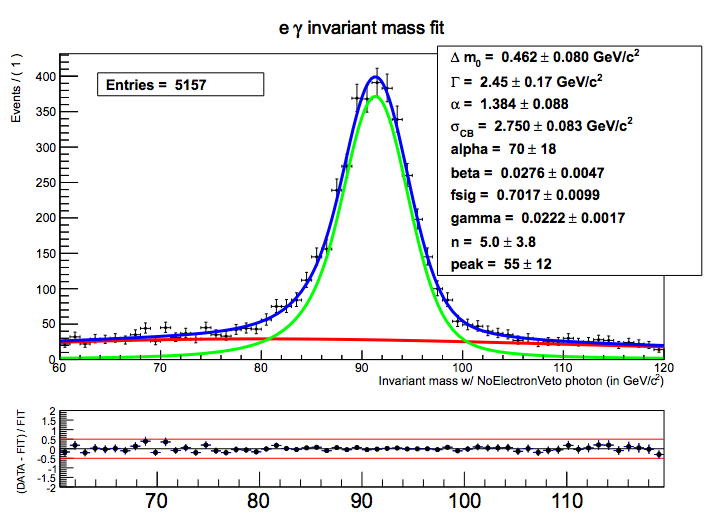
\includegraphics{ResidualDenominator_binned_negligible_errorfit}} 
       \resizebox{10cm}{!}{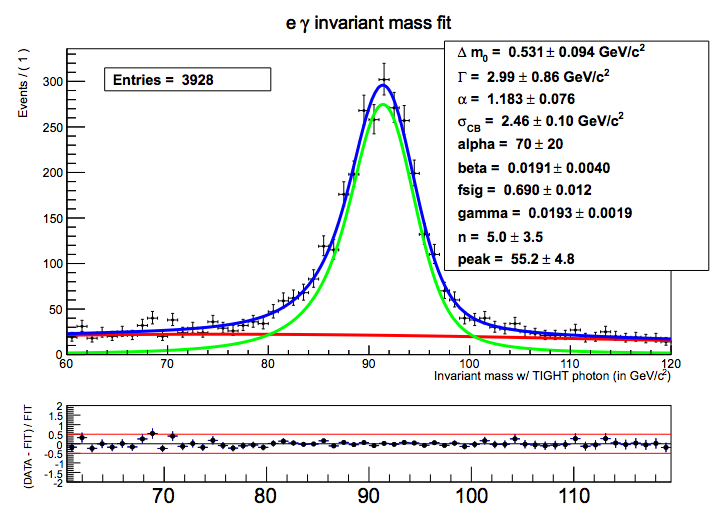
\includegraphics{ResidualNumerator_binned_negligible_errorfit}} 
  \end{center}
    \caption{Electron-Photon invariant mass fit for the no-electron-veto selection (upper plot) and the tight ID selection (lower plot). The fit fuction is a BreitWigner convoluted thanks to a fast Fourier trasformation to a 
Crystall Ball
 (for the signal) plus a CMSShape (for the background).}
    \label{Zmass_lepton}
\end{figure}

In order to count the number of fake photons for the tight and no-electron-veto selection, we use a simple Tag and Probe technique. We fit the invariant mass of an electron and a photon with a BreitWigner convoluted thanks to a 
fast Fouri
er trasformation to a Crystall Ball (for the signal) plus a CMSShape (for the background). This allows to subtract the non Drell-Yan component. The final number of fitted signal events is the number of fake photons to be used for 
the  $\e
psilon_{l}$ calculation.\\

The kinematic photon selection and event selection is the same as in the signal region. We request the jet multiplicity to be at least 4 and the transverse momentum of the photon to be 30 GeV. On the electron we apply a tight 
selection an
d we lower the transverse momenta to 20 GeV in order to get enough statistics at the low end of the invariant mass distribution. \\

The fit is performed in the invariant mass range between 60 and 120 GeV. The results of the fit are presented in Fig. \ref{Zmass_lepton}.

\subsubsubsection{Photon Fake Rate from jets}


To estimate the contribution from fake photons from jets, we use a template fitting technique. \\

First of all we define a Fakeable Object. This object is defined as an EM SuperCluster (SC) with certain characteristics:

\begin{itemize}

\item The SC has be close to a jet within a $\Delta R$ distance of 0.5. This should reduce the real photon contamination and, at the same time, it allows to have a jet of reference to which one can apply the quark-gluon tagger. We 
define 
therefore Gluon-like photons those photons for which the associated jet has a QGTagsLikelihood smaller than 0.9. While the rest of the photons will be called Quark-like.
\item The SC has to pass looser ID cuts, with respect to the tight ID selection. The ID cuts are loosened by a factor of 5.
\item The SC has to pass inverted tight ID cuts, which have been multiplied by the 2, 2, 2, 3 (for the Gluon-like) and 0, 3, 1, 0 (for the Quark-like) respectively for 1/5 of the H/E tower threshold, the charge isolation, the 
neutral isol
ation and the photon isolation cuts.

\end{itemize}

Once defined the FO, we can fit the $\sigma_{i \eta i \eta}$ distributioon of these objects thanks to a template fit and obtain the signal fraction (which in our case will determine the number of fake photons from jets) and 
subtract the b
ackground component (which will be represented by the real photons). \\

In order to perform the fit we obtain the background and signal templates respectively from data and from MC corrected with data-driven correction factors. \\

The corretions for the signal are the following:

\begin{eqnarray}
\sigma_{i \eta i \eta}^{EB corr} = (\sigma_{i \eta i \eta} - 0.0090405) \times 1.04 + 0.0089405 \nonumber \\
\sigma_{i \eta i \eta}^{EE corr} = \sigma_{i \eta i \eta} \times 1.1 - 0.0025 \nonumber \\
\end{eqnarray}

separately for the Barrel and Endcap photons. It has to be noticed that the corrections are MC sample and run dependent and have been derived for a different analysis. Therefore applying the corrections does not necesarely mean to 
use the
 correct shapes for the signal templates. Nevertheless, we have verified that applying the corrections helps the fit. Furthermore, the possible residual small differences between the true signal shapes and those used in the fit 
are taken 
into account by applying a systematic uncertainty on the shape while calculating the $\epsilon_{j}$s. \\ 

\begin{figure}[!ht]
  \begin{center}
       \resizebox{7cm}{!}{\includegraphics{Inclusive_Barrel_Sigma_Ieta_Ieta_TIGHT_Gluon.pdf}} 
       \resizebox{7cm}{!}{\includegraphics{Inclusive_Endcap_Sigma_Ieta_Ieta_TIGHT_Gluon.pdf}} 
       \resizebox{7cm}{!}{\includegraphics{Inclusive_Barrel_Sigma_Ieta_Ieta_TIGHT_Quark.pdf}} 
       \resizebox{7cm}{!}{\includegraphics{Inclusive_Endcap_Sigma_Ieta_Ieta_TIGHT_Gluon.pdf}} 
  \end{center}
    \caption{Results of the template fitting for the various FO categories: Barrel Gluon-like (uppper-left), Endcap Gluon-like (upper-right), Barrel Quark-like (lower-left) and Barrel Quark-like (lower-rigt).}
    \label{Templates}
\end{figure}


The MC process used to infer the signal templates is the photon+jets, which has trasnverse momentum spectra reasonably similar to that of the all background processes. \\

The background templates are taken directly from the data. The FO definition has been optimized to obtain a signal photon contamination fraction of less than 1$\%$. In addition we have verified that the background $\sigma_{i \eta 
i \eta}$
 shape for the FO definition and the tight ID defintion are reasonably similar using the MC. However, any possible residual difference is taken into account from the shape systematic. \\

Once obtained the shapes we can fit in the TIGHT selection the Barrel and Endcap $\sigma_{i \eta i \eta}$ distribution separately and for each FO defintion (Quark-like and Gluon-like). We perform the fit on the entire $\sigma_{i 
\eta i \e
ta}$ range, but we integrate over the tight ID $\sigma_{i \eta i \eta}$ range to obtain the number of events and the signal fraction. \\

The results are presented in Fig. \ref{Templates} and summarized in the following table:

\begin{tabular}{c c c c c}
Category    & Signal Fraction & Fit Uncertainty & Upper Edge & Lower Edge \\
\hline
Quark-like Barrel & 0.916297 & 0.000799916 & 0.934775 & 0.912988  \\
Quark-like Endcap & 0.83543  & 0.00144997  & 0.888471 & 0.789031  \\
Gluon-like Barrel & 0.941792 & 0.0022779   & 0.965953 & 0.923636  \\
Gluon-like Endcap & 0.930688 & 0.00232965  & 0.957546 & 0.919471  \\
\end{tabular}

where the Upper and Lower Edges are the higher and lower signal fraction which can be obtained by assigning the discrepancy between the data points and the fit points, either to the signal contribution or to the background 
contribution. T
his is taking into account any possible our ignorance on the knowledge of the signal and background shapes. \\

In determining the $\epsilon_{j}$s uncertainties, fit and shape uncertainties are then added in quadrature.

\subsubsubsection{Photon Signal Efficiency}

\begin{figure}[!ht]
  \begin{center}
       \resizebox{10cm}{!}{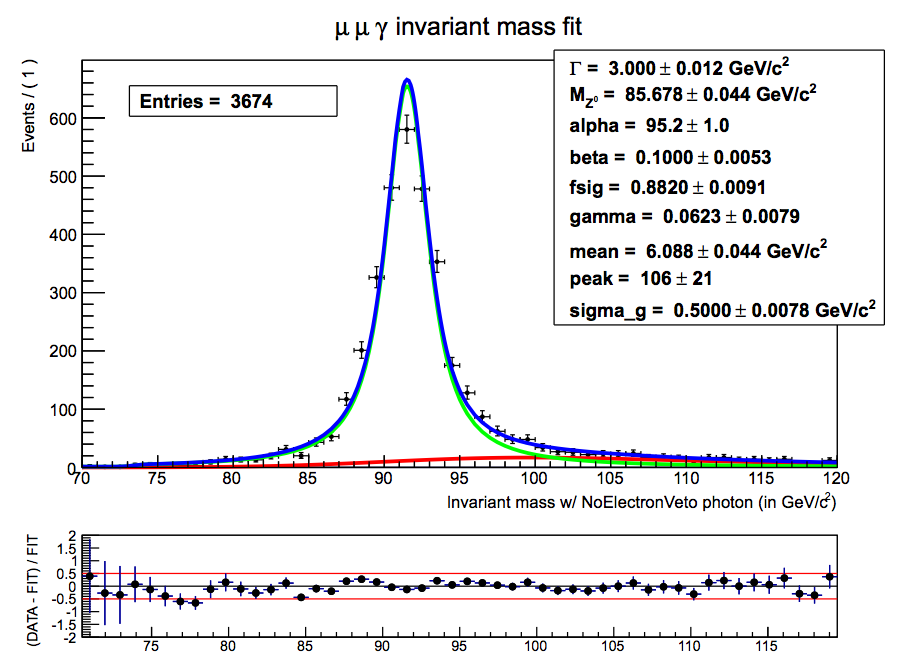
\includegraphics{Zmass_NoElectronVeto.pdf}} 
       \resizebox{10cm}{!}{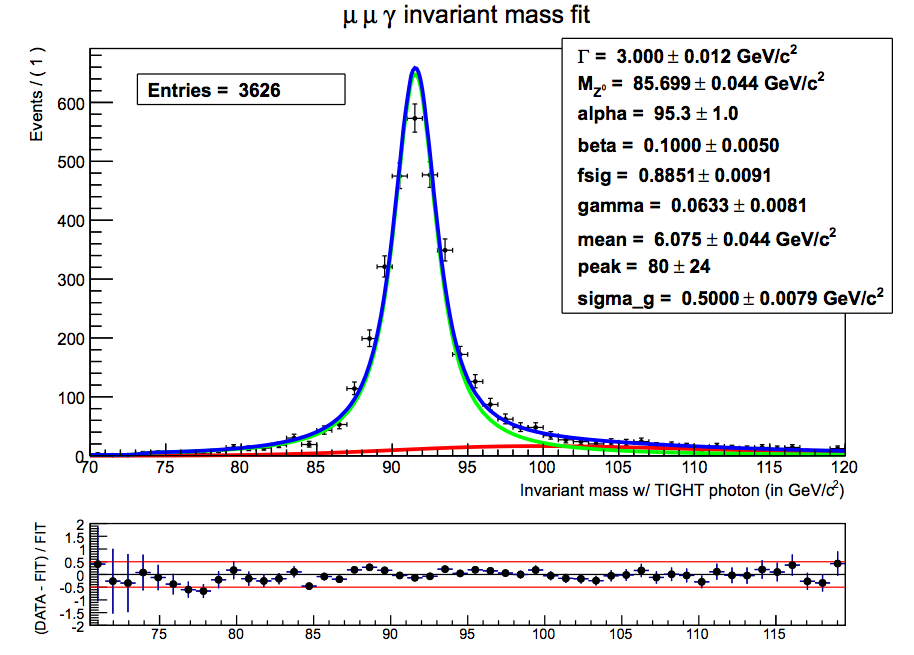
\includegraphics{Zmass_TIGHT.pdf}} 
  \end{center}
    \caption{Muon-Muon-Photon invariant mass fit for the no-electron-veto selection (upper plot) and the tight ID selection (lower plot). The fit fuction is a BreitWigner convoluted thanks to a fast Fourier trasformation to a 
Gaussian (fo
r the signal) plus a CMSShape (for the background).}
    \label{Zmass_signal}
\end{figure}

As in the case of the fake rate from leptons, also in this case we use a Tag and Prone technique. We define the $\epsilon_{s}$ as the per-object ratio of the photon efficiency for the tight selection over the sum of the 
efficiencies  for 
the no-electron-veto selection and the FO selection. However, the FO selection has been optimized to have negligible real photon contamination, therefore it will not be taken into account.

In order to count the number of fake photons for the tight and no-electron-veto selection, we use a simple Tag and Probe technique on the invariant mass of the muon-muon-photon system. \\

We fit the invariant mass with a BreitWigner convoluted thanks to a fast Fourier trasformation to a Gaussian (for the signal) plus a CMSShape for the Background. This allows to subtract the non Drell-Yan component. The final 
number of fit
ted signal events is the number of real photons to be used for the  $\epsilon_{s}$ calculation.\\

We apply no selection on the jet multiplicity to be at least 4, because we verified that the ratio of the efficiencies has no depedence on the jet multiplicity. We request the transverse momentum of the photon to be 30 GeV. On the 
leading
 muon transverse momentum we apply a tight selection and we lower the transverse momenta to 20 GeV in order to get enough statistics at the low end of the invariant mass distribution. \\

The fit is performed in the invariant mass range between 70 and 120 GeV. To increase the statistics we use both DoubleMu and SingleMu Primary Datasets, while we remove duplicated events.  The results of the fit are presented in 
Fig. \ref{Zmass_signal}.


\subsubsection{Ratio Factors}

The ratio factors are determined from the data. To determined all the ratio factors is enough to determined the following number of events: $N^{sl}_{L}$, $N^{sq}_{L}$, $N^{sg}_{L}$, $N^{qg}_{L}$, $N^{lg}_{L}$, $N^{lq}_{L}$, 
$N^{ll}_{L}$, 
$N^{qq}_{L}$, $N^{gg}_{L}$. \\

In a good approximation the above number of events can be obtained by selecting two photons events in which as $s$, $l$, $g$, $q$ photons, one can request a tight, anti-electron-veto, FO Quark-like and FO Gluon-like object, 
respectively. 
Any contamination due to this approximation can be subtracted by subtracting from MC the non-matching component (where in this case the matching is a MC matching to obtain true objects). \\

Given the FO defition used the number of two photon-like object events containing at least one FO is small. In order to increase the statistics another FO defintion has been used. The alternative FO definition has been used to 
infer the r
atio factors, after applying a correction factor which is derived from the data. The correction factor takes into account the ratio of the two FO definitions on a per-object base.  

\subsubsubsection{Results}

After having estimated the ratio factors, real photon efficiency and the fake rates the matrix can be inverted in order to obtain the $N^{ff}_{T}$ and $N^{sf}_{T}$. The uncertainties are obtained by mean of 10 M pseudo-experiments 
and by 
rejecting solutions with negative number of events. In the pseudo-experiments the ratio factors and the $\epsilon$s are let variate within their uncertainties.

The final results are: $N_{sf}^{T} =  7.9 \pm 0.4$ and $N_{ff}^{T} =  1.7  \pm 0.08$.











